% sample main.tex created 2015-03-26 by bob jantzen
\documentclass{ws-procs975x65}
% optional packages


\usepackage[T1]{fontenc}
% you should really always use T1 fonts! even as a native english writer.. see:
% http://tex.stackexchange.com/questions/664/why-should-i-use-usepackaget1fontenc

%\usepackage[utf8]{inputenc}
%\usepackage{graphicx}
\usepackage{xspace}


%%%%%%%%%%%%%%%%%%%%%%%%%%%%%%%%%%%%%%%%%%%%%%%%%%%%%%%%%%%%%%%%%%%%%%%%%%%%%%%%%
% a few author defined macros like:
%\def\beq{\begin{equation}}
%\def\eeq{\end{equation}}

%%%%%%%%%%%%%%%%%%%%%%%%%%%%%%%%%%%%%%%%%%%%%%%%%%%%%%%%%%%%%%%%%%%%%%%%%%%%%%%%%

% shortcuts for pubs
\newcommand{\apj}{ApJ}
\newcommand{\apjs}{ApJS}
\newcommand{\apjl}{ApJL}
\newcommand{\aap}{A{\&}A}
\newcommand{\aaps}{A{\&}AS}
\newcommand{\mnras}{MNRAS}
\newcommand{\aj}{AJ}
\newcommand{\araa}{ARAA}
\newcommand{\pasp}{PASP}
\newcommand{\pasj}{PASJ}
\newcommand{\nat}{Nature}
\newcommand{\nar}{New Astr Rev}


% makes it easier to have consistent writing, and easy change if needed
\newcommand{\spl}{SpaghettiLens\xspace}
\newcommand{\sw}{Space Warps\xspace}

\newcommand{\Msun}{\ensuremath{\text{M}_\odot}\xspace}

\newcommand{\Mlens}{\ensuremath{\text{M}_\text{lens}}\xspace}
\newcommand{\Mstel}{\ensuremath{\text{M}_\odot}\xspace}

% shortcut for einstein radius (Text Greek Full Math)
\newcommand{\ERf}[1][]{$\Theta_\text{E#1}$\xspace} % full output
%\newcommand{\ER}{Einstein radius\xspace} % text
%\newcommand{\ERg}[1][]{$\Theta_{\text{E#1}}$\xspace} % er in textmode with greek
%\newcommand{\ERm}[1][]{\Theta_\text{E#1}} % mathmode with greek symbol
%\newcommand{\kenc}[1][r]{$\kappa_\text{encl}(#1)$\xspace}
%\newcommand{\kap}[1][r]{$\kappa(#1)$\xspace}

% shorcuts for refs and citations
\newcommand{\icite}[1]{Ref.~\refcite{#1}}  % Direct *I*nline citation
\newcommand{\ccite}[1]{(see \icite{#1})}   % ``(see Ref~ref)'' type citation
\newcommand{\scite}[1]{\cite{#1}}          % end of *S*entence citation

\newcommand{\figref}[1]{Fig.~\ref{fig:#1}}

%\newcommand{\fref}[1]{\ref{fig:#1}}
%\newcommand{\sref}[1]{\ref{sec:#1}}
%\newcommand{\tref}[1]{\ref{tab:#1}}
%\newcommand{\secref}[1]{Section~\ref{sec:#1}}
%\newcommand{\tabref}[1]{Table~\ref{tab:#1}}
%\newcommand{\Figref}[1]{Figure~\ref{fig:#1}}
%\newcommand{\Secref}[1]{Section~\ref{sec:#1}}
%\newcommand{\Tabref}[1]{Table~\ref{tab:#1}}


% shortcut for ASW000xxxx
\newcommand{\asw}[1]{ASW000#1\xspace}
\newcommand{\model}[2][Model~]{#1#2\xspace}


\newcommand{\dgr}{^{\circ}}
\newcommand{\tgeom}{t_{\rm geom}}
\newcommand{\tgrav}{t_{\rm grav}}
\newcommand{\subcirc}{{\lower.33ex\hbox{$\circ$}}}
\newcommand{\subbullet}{{\lower.33ex\hbox{$\bullet$}}}




\begin{document}



\title{Lensing galaxies in the CFHT Legacy Survey}

\author{
  Rafael K\"ung$^*$, Prasenjit Saha
}
\address{
Physik-Institut, University of Zurich,\\
Winterthurerstrasse 190, 8057 Zurich, Switzerland\\
$^*$E-mail: rafael\_kueng@uzh.ch
}
\author{
  Anupreeta More, Surhud More
}
\address{
  Kavli Institute for the Physics and Mathematics of the Universe, University of Tokyo\\ 5-1-5 Kashiwanoha, Kashiwa-shi 277-8583, Japan
}

\author{
  Elisabeth Baeten, Claude Cornen, Christine Macmillan, Julianne K. Wilcox
}
\address{
  Zooniverse, c/o Astrophysics Department, University of Oxford\\
  Oxford OX1 3RH, UK
}

\author{
  Jonathan Coles
}
\address{
  Exascale Research Computing Lab, Campus Teratec,\\
  2 Rue de la Piquetterie, 91680 Bruyeres-le-Chatel, France
}

\author{Ignacio Ferreras}
\address{Mullard Space Science Laboratory, University College London, Holmbury St Mary, Dorking, Surrey RH5 6NT, UK}

\author{
  Phil Marshall
}
\address{
  Kavli Institute for Particle Astrophysics and Cosmology, Stanford University\\
  452 Lomita Mall, Stanford, CA 94035, USA
}

\author{
  Aprajita Verma
}
\address{
  Sub-department of Astrophysics, University of Oxford, Denys Wilkinson Building\\
  Keble Road, Oxford, OX1 3RH, UK
}






\begin{abstract}
In SpaceWarps, a community of over 30\,000 % note: SI rules forbid to use , or . for separation of 1000th (9. conference, 1948, Resolution 7) http://www.bipm.org/en/CGPM/db/9/7/
volunteers searched for lensed candidates in the CFHT Legacy Survey.
59 new lens candidates have been identified, along with rediscovery of 60\% of the previously-known candidates.

Models of most of these lens candidates were produced collaboratively by a small community of lens enthusiasts from the volunteer community.
Tests with simulated lenses show that models by experienced volunteers are comparable to those by experts.
We present lens models of some of these newly discovered lens candidates, along with a modelling method developed to be usable in a citizen-science environment.
\end{abstract}


\keywords{Gravitational Lensing: strong; methods: numerical}


\bodymatter

%%%%%%%%%%%%%%%%% now a standard article style for the most part


\section{Introduction}

Gravitational lenses, predicted by A. Einstein's General Relativity in 1915 have become an important tool in cosmology.
Strong lensing can be used to infer the distribution of dark matter around galaxies \ccite{Koopans2009}, to find the relation between stars and dark matter \ccite{Leier2011} or to infer cosmological parameters \ccite{Sereno2014}.

Current surveys resulted in more than 400 known lenses.
For example in the \sw project, carried out on the 170 square degree Canada--France--Hawaii Telescope Legacy Survey (CFHTLS), over 30\,000 volunteers found 59 candidate lenses.\scite{sw1,sw2}

As a rough estimate, this results in one lens every few square degree.
Imaging surveys under way will increase the observation area by a factor of ten and next generation surveys starting in the twenty--twenties will increase the resolution leading to another increase by a factor of ten.\scite{Marshall2005,OguriMarshall2010}
This raises expectations that the number of lenses will increase a hundred fold, leading to an order of 10\,000 lenses over the next 10 years.
That's of order one potential lens detection per hour for the next 10 years.

Software robots in combination with the citizen science project \sw are proposed to classify that amount of raw data and identify possible lens candidates.\scite{Marshall2009,sw1}
For the modelling of the mass distribution of the lenses --- an essential part of any research involving lenses --- we propose to involve citizen scientists as well and present a concept, that has already been implemented and tested: \spl.\scite{Kueng2015}


\section{Theoretical background and implementation}

This section is a short summary from \icite{Kueng2015} and recaps the basic concepts of \spl.
It follows the formulation of Fermat's principle as described in \icite{Blandford1986}.

Consider a lens at redshift $z_L$ away from the observer with a planar mass distribution proportional to $\kappa(x,y)$, the convergence.
Imagine a light source at distance $z_s$, behind the point $(x_s,y_s)$ on the lens.
A photon flying from the source through the lens at $(x,y)$ to the observer will have an increased light travel time compared to the direct way through $(x_s,y_s)$.
The time delay can be expressed as two parts:
\begin{equation}  \label{eq:tarriv}
t(x,y) = t_{\rm geom} + t_{\rm grav} ,
\end{equation}
where the first part represents a geometrical time delay,
\begin{equation} \label{eq:tgeom}
\tgeom(x,y) \propto (x-x_s)^2 + (y-y_s)^2 ,
\end{equation}
and the second the delay due to general relativity:
\begin{equation} \label{eq:tgrav}
\tgrav(x,y) = \left\langle \tgrav(x_\subcirc,y_\subcirc) \right\rangle
              + (1+z_L) \frac{2G}{c^3} M(x_\subbullet,y_\subbullet) \,.
\end{equation}

The arrival time surface $t(x,y)$ applies to virtual photons.
Real photons take paths where $t(x,y)$ is stationary, due to Fermat's principle.
This arrival time surface has an exact relation to the lens-mass distribution and the source position.
A simple sketch of this surface (i.e. the location of minima, maxima and saddle points, and the self intersection contour though saddle points) is thus a sufficient starting point for finding a lensing mass distribution $\kappa(x,y)$. Further details about the Metropolis-Hastings sampling technique are described in \icite{Lubini2012}.
What is called a \spl model is actually an ensemble of 200 models, each a possible solution to the constraints. The uncertainty is the range of parameters covered by all the models of the whole ensemble.


\section{Analysing the \sw candidates}

(too tired to write any good text now..
something about that each candidate got modlelled multiple times, models were improved, and finally the best was selected) Sample tree of models is depicted in \figref{tree}

for this analysis, models from the tree were selected manually by inspection by PS, RK and the community.

\begin{figure}
  \centering
  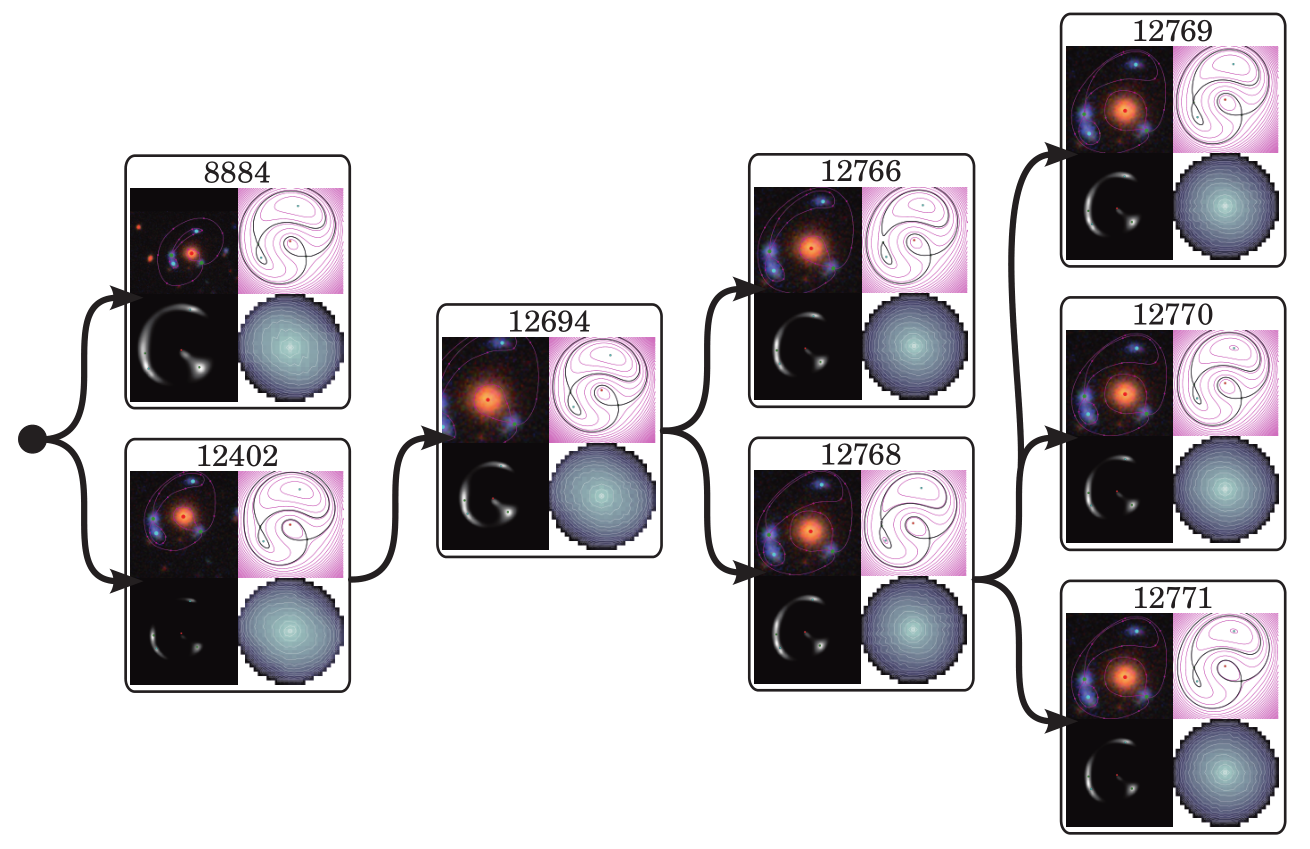
\includegraphics[width=\columnwidth]{img/modeltree}
  \caption{
    Tree of models for the lens candidate SW5 (J143454.4+522850)
  }
  \label{fig:tree}
\end{figure}



\subsection{Determing lensing and stellar mass}

In a next step, we extracted the total lensing mass and the stellar mass and compared the ratio, to get a first overview over the condidates and to reject possible non--lenses.

The lensing mass can directly be extracted from the generated models, as the mass distribution is the key feature that is being modelled \icite{Kueng2015}.
Since a single model actually consists of an ensemble of a number of models, where each one is a possible configuration, we get an approximation of the error by selecting the models with minimal/ maximal total mass as lower / upper bounds for the errors.

We estimated the stellar mass with:
\[
  \Mstel = 10^{0.4 [\operatorname{mag}(z_\text{ph}) - m_\text{i}]}
\]
where
$z_\text{ph}$ and $m_\text{i}$ are the photometric redshift and luminosity given in \icite{sw2} and 
$\operatorname{mag}()$ is a function obtained by interpolating data of SDSS-i magnitude (AB) of 1\Msun and actual mass vs redshift BC03 models \icite{Bruzual2003}, Salpeter Initial Mass Function and assumes ``vanilla cosmology'' ($\Omega_\text{M}=0.3$, $\Omega_\Lambda=0.7$).\scite{Ferreras2010}
For the lower bound of the error we assumed a young population (0.5 Gyr), whereas for the upper one of 2 Gyr.

\begin{figure}
  \centering
  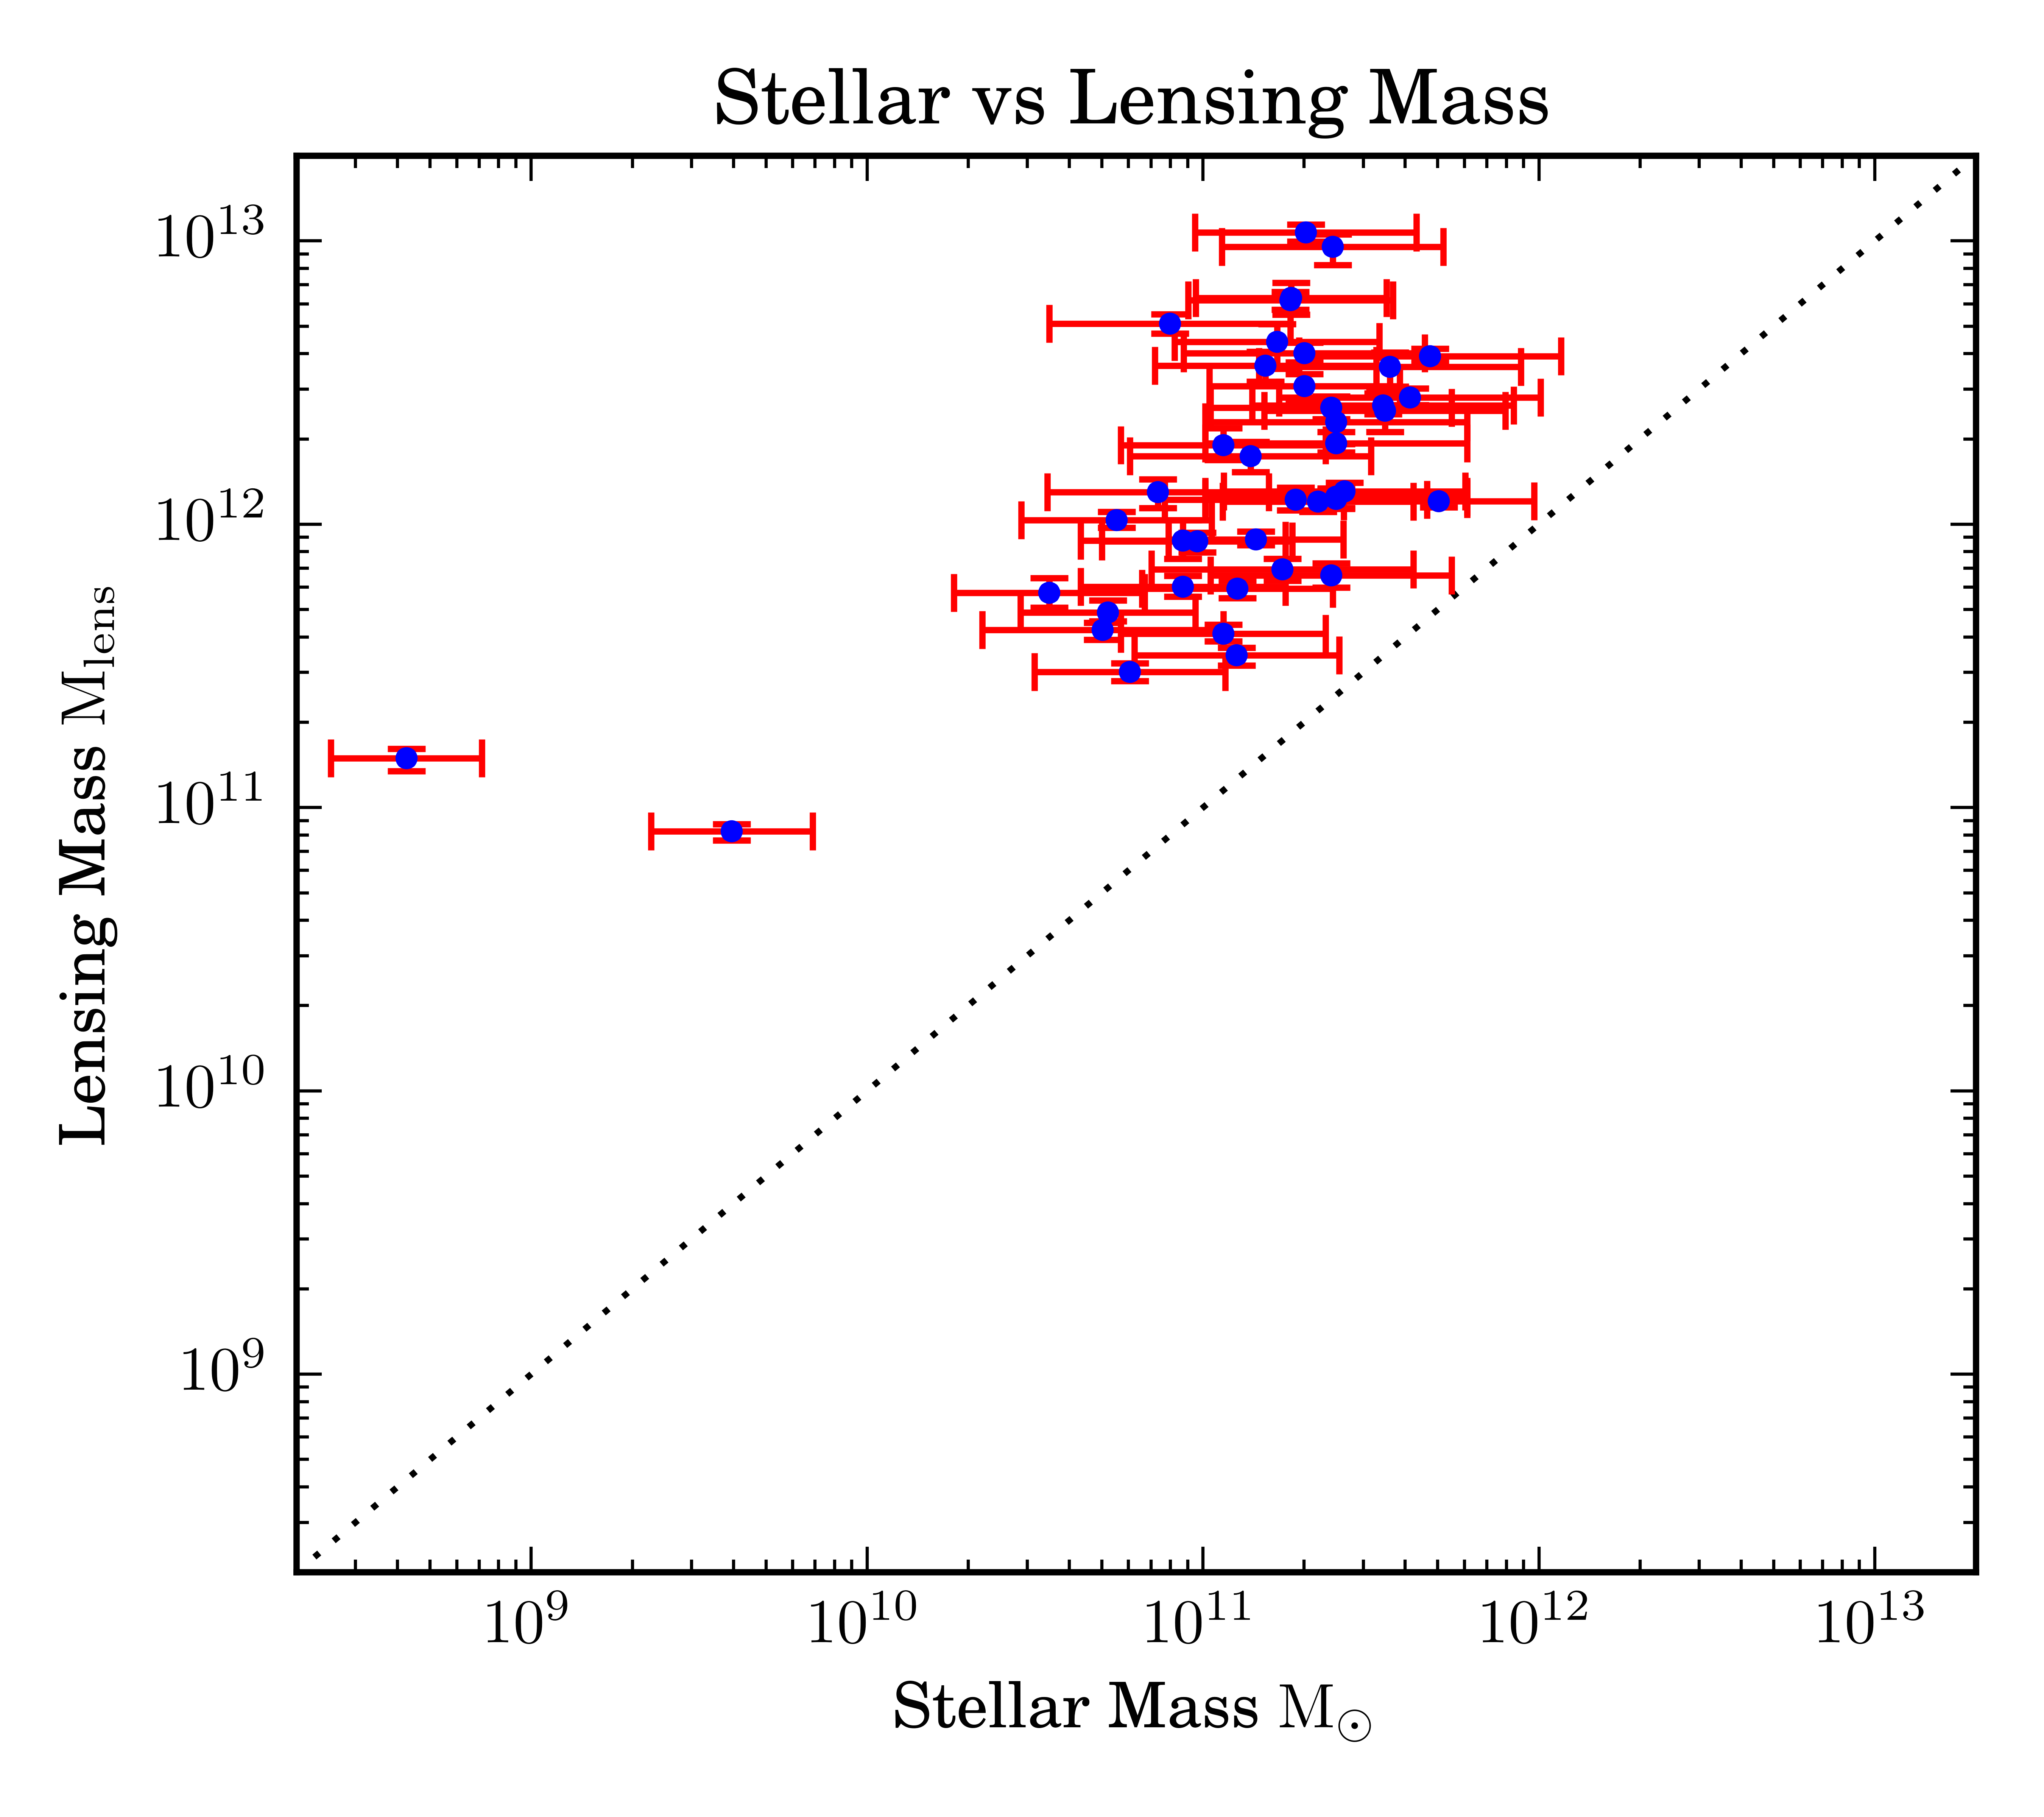
\includegraphics[width=0.8\columnwidth]{img/plot}
  \caption{Stellar Mass \Mstel vs. Lensing Mass \Mlens. Stellar Mass errors are the difference between junior (0.5 Gyr) and senior (2 Gyr) population; Lensing Mass errors represent the minimum and maximum values of an ensemble (``a model'').}
  \label{fig:frac}
\end{figure}


\section{Conclusions}

In this work we use the method presented and tested in \icite{Kueng2015} to create models of all lens candidates discovered by the first run of \sw\icite{sw2}.
We determine the total (lensing) mass \Mlens of the candidates using the generated models and the stellar mass \Mstel using an interpolation of a Salpeter Initial Mass Function \icite{Salpeter1955} with redshifts and luminosity magnitudes given in \icite{sw2}.
We then plot the masses of the candidates and observe in \figref{frac} that the stellar mass fraction is of the order of 20\%, with decreasing trend for the most massive galaxies, as expected for early type galaxies.
We identify outliers with very low stellar masses that need further inspection.


\section*{Acknowledgments}
RK thanks the Candoc Forschungskredit of the University of Zurich for the support of this work.

\bibliographystyle{ws-procs975x65}
\bibliography{ms}



% \section{The First Section: Titles are Capitalized with the Usual First Letter Rules}
% \subsection{Subsections only have the first letter of the entire title capitalized}
% 
% Subsections only have the first letter of the first word capitalized (except for words that are naturally capitalized). For a very short contribution it is not necessary to use the sectioning commands.
% 
% You may also use the ``graphicx" package and use its related commands if you are already familiar with that figure insertion method. Word template files are discouraged, allowed as a last resort for those people who have some difficulties with \LaTeX.
% 
% Since the World Scientific proceedings style \cite{ws} uses numbered superscript citations of the bibliography items, one has to be careful to use 
% \verb|\refcite| to get a baseline normal size number to include in an in-line direct reference, best formatted in the style: 
%  ``see Ref.$\sim$\verb|\refcite|\{\ldots\}" while normal superscript citations follow punctuation  as in ``.\verb|\cite|\{\ldots\}"  For example, here is an in line citation to Ref.~\refcite{arxiv}. On the other hand citations at the end of a sentence are done line this.\cite{lamp94}
% 
% \subsection{You can safely ignore this}
% 
% The white space above the title in the ws-procs975x65.cls document style is eliminated by commenting out two lines in the definition of the macro \verb|\title|, namely:\\  
%  \verb|\vspace|*\{-14pt\} \\ \verb|\vskip| 59pt\\
% but you do not need to know this if you use the proceedings style files downloaded from the MG14 website. This gives a bit more space for text content in short articles.
% 
% For MG14 \cite{mg14} only a preview PDF document will be collected (exported from your \LaTeX\ document) before the meeting takes place.
% 
% \section*{Acknowledgments}
% 
% What a debt we all owe to Donald Knuth for his gift of \TeX\ to us and to Leslie Lamport as well for its \LaTeX\ child.



\end{document}

